%% phase_N3_report.tex
%% Self-contained report on Phase N3: Asian Option Refinement Study (SIAM)
%% Compile with: pdflatex phase_N3_report.tex
%%
\documentclass[11pt,a4paper]{article}

\usepackage{amsmath, amssymb, amsthm}
\usepackage{booktabs}
\usepackage{graphicx}
\usepackage{geometry}
\usepackage{hyperref}
\usepackage{microtype}
\usepackage{xcolor}
\usepackage{caption}
\usepackage{subcaption}
\usepackage{enumitem}
\usepackage{multirow}
\usepackage{array}

\geometry{margin=2.5cm}
\emergencystretch=2.5em

\hypersetup{
  colorlinks=true, linkcolor=blue!60!black,
  citecolor=blue!60!black, urlcolor=blue!60!black
}

\newcommand{\Nz}{N_z}
\newcommand{\Nt}{N_t}
\newcommand{\bigo}[1]{\mathcal{O}(#1)}
\newcommand{\half}{\tfrac{1}{2}}
\newcommand{\Uex}{U_{\rm exact}}
\newcommand{\MC}{\mathrm{MC}}

% ------------------------------------------------------------------
\title{\textbf{Phase N3: Asian Option Refinement Study}\\
       \large V6 Rogers--Shi Solver --- Spatial, Temporal, Domain
       and Boundary-Condition Analysis}
\author{dpg-finance project}
\date{2026-05-28 \quad (commit \texttt{e7c0a7d})}
% ------------------------------------------------------------------

\begin{document}
\maketitle
\tableofcontents
\bigskip

% ==================================================================
\section{Objective}
% ==================================================================

Phase~N3 performs a systematic refinement study for the V6 primal DPG
solver applied to the Rogers--Shi reduced arithmetic-average Asian call.
The study goes beyond the benchmark table of Phase~C by separating four
distinct sources of error:

\begin{enumerate}[noitemsep]
  \item \textbf{Spatial discretization} (N3-A1): mesh refinement in $\Nz$
        at fixed $\Nt = 800$.
  \item \textbf{Temporal discretization} (N3-A2): time-step refinement in
        $\Nt$ at fixed $\Nz = 800$.
  \item \textbf{Domain truncation} (N3-A3): sensitivity to the computational
        domain $[-D,D]$ for $D \in \{2,3,4,5\}$.
  \item \textbf{Boundary conditions} (N3-A4): four boundary-condition
        variants on the same domain $[-2,2]$.
\end{enumerate}
In addition, N3-A5 targets the parameter combination that exhibited the
largest error in the Phase~C benchmark table and studies its behaviour
under spatial refinement up to $\Nz = 1600$.

All DPG prices are compared against a Monte Carlo benchmark for the
arithmetic-average fixed-strike Asian call.

% ==================================================================
\section{Mathematical Model}
% ==================================================================

\subsection{Rogers--Shi substitution}

Following Rogers and Shi~\cite{rs1995}, the change of variable
\[
  z(t) = \frac{K - A(t)/T}{S(t)},
  \qquad
  A(t) = \int_0^t S(s)\,\mathrm{d}s,
\]
reduces the pricing PDE for the arithmetic-average Asian call to a
one-dimensional degenerate parabolic equation.  With backward time
$\tau = T - t$, the normalised price $U(\tau, z) = V/S_0$ satisfies
\begin{equation}
  \frac{\partial U}{\partial\tau}
  - \frac{\sigma^2}{2}\,z^2\,\frac{\partial^2 U}{\partial z^2}
  + \left(\frac{1}{T} + rz\right)\frac{\partial U}{\partial z} = 0,
  \quad
  (\tau, z) \in (0, T] \times (z_{\min}, z_{\max}),
  \label{eq:pde}
\end{equation}
with terminal condition (IC in backward time)
\begin{equation}
  U(0, z) = \max(0, -z),
  \label{eq:ic}
\end{equation}
homogeneous Dirichlet BC $U = 0$ at $z = z_{\max}$ (right boundary), and
a natural (zero-flux) condition at $z = z_{\min}$ (left boundary).
The diffusion coefficient $(\sigma^2/2)z^2$ vanishes at $z = 0$, making
the problem \emph{degenerate}.  The option price is recovered as
\[
  V = S_0 \cdot U(T,\, z_0), \qquad z_0 = K/S_0.
\]

\subsection{Galerkin bilinear form}

Integration by parts on the variable-coefficient diffusion term
$-(\sigma^2/2)z^2 U_{zz}$ introduces an effective convection coefficient.
The primal DPG bilinear form at each time step (backward Euler with
time step $\Delta\tau = T/\Nt$) is
\[
  a(U, v)
  = \frac{1}{\Delta\tau}(U, v)
  + \frac{\sigma^2}{2}\,z^2\,(U_z,\, v_z)
  + \left[\frac{1}{T} + (r + \sigma^2)z\right](U_z,\, v),
\]
where the effective convection $1/T + (r+\sigma^2)z$ absorbs the
IBP correction $\sigma^2 z$ from $\partial_z[(\sigma^2/2)z^2]$.

\subsection{Monte Carlo benchmark}

All DPG prices are compared against the Monte Carlo estimator
\begin{equation}
  V_{\MC} = e^{-rT}\,\mathbb{E}\!\left[\max\!\left(\bar{S} - K,\, 0\right)\right],
  \qquad
  \bar{S} = \frac{1}{T}\int_0^T S(t)\,\mathrm{d}t,
  \label{eq:mc}
\end{equation}
simulated by Euler--Maruyama with $n_{\rm paths}$ paths and
$n_{\rm steps}$ time steps, seed 42.  The 95\% confidence interval is
$V_{\MC} \pm 1.96\,\mathrm{SE}$, where
$\mathrm{SE} = e^{-rT}\,\mathrm{std}(\text{payoffs})/\sqrt{n_{\rm paths}}$.

% ==================================================================
\section{Experimental Parameters}
% ==================================================================

All experiments use $S_0 = 100$, $T = 1$, $r = 0.09$, and $H^1(p=1)$
finite elements.  Default domain is $[-2, 2]$ unless stated otherwise.
Table~\ref{tab:params} summarises the study design.

\begin{table}[htbp]
\centering
\caption{Study design: Phase N3 experiments.}
\label{tab:params}
\small
\begin{tabular}{@{}p{1.4cm}p{3.0cm}p{6.0cm}p{3.5cm}@{}}
\toprule
Step & Description & Varied & Fixed \\
\midrule
N3-A1 & Spatial refinement &
  $\Nz \in \{50,100,200,400,800\}$;
  $\sigma \in \{0.05,0.10,0.20,0.30\}$;
  $K \in \{95,100,105\}$ &
  $\Nt = 800$ \\[4pt]
N3-A2 & Temporal refinement &
  $\Nt \in \{50,100,200,400,800\}$;
  $\sigma \in \{0.10,0.20,0.30\}$ &
  $\Nz = 800$, $K = 100$ \\[4pt]
N3-A3 & Domain truncation &
  $D \in \{2,3,4,5\}$; $h \approx 0.02$ const. &
  $\sigma = 0.20$, $K = 100$, $\Nt = 400$ \\[4pt]
N3-A4 & BC sensitivity &
  4 variants (Table~\ref{tab:bc}) &
  $\sigma = 0.20$, $K = 100$,
  $\Nz = 400$, $\Nt = 400$ \\[4pt]
N3-A5 & Worst-case refinement &
  $\Nz \in \{200,400,800,1600\}$ &
  $\sigma = 0.05$, $K = 100$, $\Nt = 800$ \\
\bottomrule
\end{tabular}
\end{table}

The spatial EOC (Tables~\ref{tab:spatial-atm} and~\ref{tab:worst}) is
computed against the \emph{spatial self-reference} (finest $\Nz$ in the
sequence for each $(\sigma, K)$ group), not against the MC benchmark.
This separates the spatial convergence rate from the backward-Euler
temporal floor $(\bigo{\Delta\tau}$ with $\Nt = 800$), which dominates
the MC-referenced error at fine $\Nz$.  The \texttt{abs\_error} column
and \texttt{rel\_error} in all CSVs retain the MC-based quantity.

% ==================================================================
\section{N3-A1: Spatial Refinement}
% ==================================================================

\subsection{Setup}

Mesh spacing $h = 4/\Nz$ (domain width 4).  MC reference:
$n_{\rm paths} = 500{,}000$, $n_{\rm steps} = 500$, seed 42.
Temporal steps $\Nt = 800$ held fixed.  ATM ($K = 100$) results are
the primary focus; $K = 95$ and $K = 105$ are supplementary.

\subsection{Results for ATM ($K = 100$)}

Table~\ref{tab:spatial-atm} gives the full refinement table for
$\sigma \in \{0.10, 0.20, 0.30\}$, $K = 100$.

\begin{table}[htbp]
\centering
\caption{Asian ATM spatial refinement, $K = 100$, $r = 0.09$, $\Nt = 800$.
         MC reference: $n = 500{,}000$, $n_{\rm steps} = 500$, seed 42.
         EOC is spatial self-reference based (see text).
         ${}^*$ denotes the finest $\Nz$ (the spatial reference; EOC not defined).}
\label{tab:spatial-atm}
\small
\begin{tabular}{rrrrrrrr}
\toprule
$\Nz$ & $h$ & DPG price & MC ref.\ & abs.\ err. & rel.\ err.\ (\%) & EOC \\
\midrule
\multicolumn{7}{l}{$\sigma = 0.10$} \\
\midrule
   50 & 0.0800 & 5.29337 & 4.92833 & $3.650\times10^{-1}$ & 7.41 & --- \\
  100 & 0.0400 & 5.12834 & 4.92833 & $2.000\times10^{-1}$ & 4.06 & $-0.12$ \\
  200 & 0.0200 & 5.20038 & 4.92833 & $2.720\times10^{-1}$ & 5.52 & $2.62$ \\
  400 & 0.0100 & 5.21190 & 4.92833 & $2.836\times10^{-1}$ & 5.75 & $2.52$ \\
  800$^*$ & 0.0050 & 5.21434 & 4.92833 & $2.860\times10^{-1}$ & 5.80 & --- \\
\midrule
\multicolumn{7}{l}{$\sigma = 0.20$} \\
\midrule
   50 & 0.0800 & 7.03792 & 6.79268 & $2.452\times10^{-1}$ & 3.61 & --- \\
  100 & 0.0400 & 6.93681 & 6.79268 & $1.441\times10^{-1}$ & 2.12 & $1.28$ \\
  200 & 0.0200 & 6.95993 & 6.79268 & $1.672\times10^{-1}$ & 2.46 & $2.21$ \\
  400 & 0.0100 & 6.96506 & 6.79268 & $1.724\times10^{-1}$ & 2.54 & $2.36$ \\
  800$^*$ & 0.0050 & 6.96631 & 6.79268 & $1.736\times10^{-1}$ & 2.56 & --- \\
\midrule
\multicolumn{7}{l}{$\sigma = 0.30$} \\
\midrule
   50 & 0.0800 & 9.03613 & 8.84880 & $1.873\times10^{-1}$ & 2.12 & --- \\
  100 & 0.0400 & 8.94145 & 8.84880 & $9.265\times10^{-2}$ & 1.05 & $2.01$ \\
  200 & 0.0200 & 8.95593 & 8.84880 & $1.071\times10^{-1}$ & 1.21 & $2.12$ \\
  400 & 0.0100 & 8.95941 & 8.84880 & $1.106\times10^{-1}$ & 1.25 & $2.33$ \\
  800$^*$ & 0.0050 & 8.96027 & 8.84880 & $1.115\times10^{-1}$ & 1.26 & --- \\
\bottomrule
\end{tabular}
\end{table}

\subsection{Temporal error floor}

The dominant feature of Table~\ref{tab:spatial-atm} is that the
\emph{MC-referenced} absolute error \emph{does not decrease} for
$\Nz \ge 200$.  This is a \textbf{temporal error floor}: with
$\Nt = 800$ and backward Euler, the temporal discretisation error
at $\Nt = 800$ is approximately $0.18$ (see Section~\ref{sec:temporal}),
which dwarfs the spatial error at $\Nz = 200$--$800$.

The spatial convergence is clearly visible when measured against the
finest-$\Nz$ self-reference.  For $\sigma = 0.20$, $K = 100$:
\begin{itemize}[noitemsep]
  \item $\Nz = 50 \to 100$: spatial error $0.072 \to 0.029$,
        EOC $= 1.28$;
  \item $\Nz = 100 \to 200$: spatial error $0.029 \to 0.006$,
        EOC $= 2.21$;
  \item $\Nz = 200 \to 400$: spatial error $0.006 \to 0.001$,
        EOC $= 2.36$.
\end{itemize}
The EOC accelerates from $\approx 1.3$ at the coarsest refinement to
$\approx 2.4$ at the finest, consistent with improved resolution of the
kink in the initial condition $U(0, z) = \max(0, -z)$ at $z = 0$.

\subsection{Effect of $\sigma$ on spatial convergence}

For $\sigma = 0.30$ the spatial EOC (2.01, 2.12, 2.33) is essentially
$\bigo{h^2}$ from the outset, as the larger diffusion coefficient
$(\sigma^2/2)z^2$ smooths the kink more rapidly.  For $\sigma = 0.10$
(more convection-dominated), the price oscillates around the spatial
limit before settling: from $5.293$ at $\Nz = 50$ to $5.128$ at
$\Nz = 100$ (overshoots below), then converges monotonically to $5.214$
from $\Nz = 200$ onwards.  This non-monotone behaviour at the coarsest
meshes is due to the higher P\'eclet number, and the spatial EOC
recovers to $> 2.5$ for $\Nz \ge 200$.

\subsection{$\sigma = 0.05$: convection-dominated regime}

For $\sigma = 0.05$, the ATM ($K = 100$) case has a MC-referenced
relative error near $7\%$ at all mesh sizes (Table~\ref{tab:sigma005}),
again dominated by temporal error.  The OTM case ($K = 105$) has even
larger relative error ($> 69\%$) because the exact price ($\approx 0.96$)
is small and the DPG solution at these parameters has a large temporal
bias.  The ITM case ($K = 95$) performs well, with the error falling from
$8\%$ at $\Nz = 50$ to $< 0.2\%$ by $\Nz = 200$.

\begin{table}[htbp]
\centering
\caption{Spatial refinement for $\sigma = 0.05$ (convection-dominated),
         $r = 0.09$, $\Nt = 800$. MC: $n = 500{,}000$, seed 42.
         Large errors for $K = 100, 105$ are temporal in origin.}
\label{tab:sigma005}
\small
\begin{tabular}{rrrrrr}
\toprule
$K$ & $\Nz$ & DPG price & MC ref.\ & abs.\ err. & rel.\ err.\ (\%) \\
\midrule
95  &   50 & 8.11226 & 8.82183 & $7.096\times10^{-1}$ & 8.04 \\
95  &  100 & 8.72709 & 8.82183 & $9.475\times10^{-2}$ & 1.07 \\
95  &  200 & 8.83622 & 8.82183 & $1.439\times10^{-2}$ & 0.16 \\
95  &  400 & 8.83209 & 8.82183 & $1.026\times10^{-2}$ & 0.12 \\
95  &  800 & 8.83298 & 8.82183 & $1.115\times10^{-2}$ & 0.13 \\
\midrule
100 &   50 & 4.71324 & 4.32066 & $3.926\times10^{-1}$ & 9.09 \\
100 &  100 & 4.44072 & 4.32066 & $1.201\times10^{-1}$ & 2.78 \\
100 &  200 & 4.59510 & 4.32066 & $2.744\times10^{-1}$ & 6.35 \\
100 &  400 & 4.61938 & 4.32066 & $2.987\times10^{-1}$ & 6.91 \\
100 &  800 & 4.62316 & 4.32066 & $3.025\times10^{-1}$ & 7.00 \\
\midrule
105 &   50 & 2.01703 & 0.96460 & $1.052\times10^{0}$  & 109.1 \\
105 &  100 & 1.72662 & 0.96460 & $7.620\times10^{-1}$ & 79.0 \\
105 &  200 & 1.65727 & 0.96460 & $6.927\times10^{-1}$ & 71.8 \\
105 &  400 & 1.63263 & 0.96460 & $6.680\times10^{-1}$ & 69.3 \\
105 &  800 & 1.63618 & 0.96460 & $6.716\times10^{-1}$ & 69.6 \\
\bottomrule
\end{tabular}
\end{table}

% ==================================================================
\section{N3-A2: Temporal Refinement}
\label{sec:temporal}
% ==================================================================

\subsection{Setup}

Fix $\Nz = 800$ (fine spatial mesh), $K = 100$, $r = 0.09$, domain
$[-2, 2]$.  Vary $\Nt \in \{50, 100, 200, 400, 800\}$ for
$\sigma \in \{0.10, 0.20, 0.30\}$.  MC reference:
$n_{\rm paths} = 1{,}000{,}000$, $n_{\rm steps} = 1000$, seed 42
(higher fidelity than N3-A1 to reduce MC noise in the EOC).

\subsection{Results}

Table~\ref{tab:temporal} shows the temporal refinement data.

\begin{table}[htbp]
\centering
\caption{Asian temporal refinement, $K = 100$, $r = 0.09$, $\Nz = 800$.
         MC: $n = 1{,}000{,}000$, $n_{\rm steps} = 1000$, seed 42.
         EOC$_t = \log(e_{i-1}/e_i)/\log(\Nt_i/\Nt_{i-1})$.}
\label{tab:temporal}
\small
\begin{tabular}{rrrrrrrr}
\toprule
$\sigma$ & $\Nt$ & $\Delta\tau$ & DPG price & MC ref.\ & abs.\ err. & rel.\ err.\ (\%) & EOC$_t$ \\
\midrule
0.10 & MC & & & $4.9210$ & & & \\
\midrule
0.10 &  50 & 0.0200 & 8.23406 & 4.9210 & $3.313$ & 67.3 & --- \\
0.10 & 100 & 0.0100 & 6.86724 & 4.9210 & $1.946$ & 39.5 & $0.77$ \\
0.10 & 200 & 0.0050 & 6.00473 & 4.9210 & $1.084$ & 22.0 & $0.85$ \\
0.10 & 400 & 0.0025 & 5.49561 & 4.9210 & $5.746\times10^{-1}$ & 11.7 & $0.92$ \\
0.10 & 800 & 0.0013 & 5.21434 & 4.9210 & $2.934\times10^{-1}$ &  5.96 & $0.97$ \\
\midrule
0.20 & MC & & & $6.7830$ & & & \\
\midrule
0.20 &  50 & 0.0200 & 9.26221 & 6.7830 & $2.479$ & 36.5 & --- \\
0.20 & 100 & 0.0100 & 8.14515 & 6.7830 & $1.362$ & 20.1 & $0.86$ \\
0.20 & 200 & 0.0050 & 7.50075 & 6.7830 & $7.177\times10^{-1}$ & 10.6 & $0.92$ \\
0.20 & 400 & 0.0025 & 7.14992 & 6.7830 & $3.669\times10^{-1}$ &  5.41 & $0.97$ \\
0.20 & 800 & 0.0013 & 6.96631 & 6.7830 & $1.833\times10^{-1}$ &  2.70 & $1.00$ \\
\midrule
0.30 & MC & & & $8.8351$ & & & \\
\midrule
0.30 &  50 & 0.0200 & 10.72093 & 8.8351 & $1.886$ & 21.3 & --- \\
0.30 & 100 & 0.0100 &  9.82943 & 8.8351 & $9.943\times10^{-1}$ & 11.3 & $0.92$ \\
0.30 & 200 & 0.0050 &  9.34402 & 8.8351 & $5.089\times10^{-1}$ &  5.76 & $0.97$ \\
0.30 & 400 & 0.0025 &  9.09013 & 8.8351 & $2.550\times10^{-1}$ &  2.89 & $1.00$ \\
0.30 & 800 & 0.0013 &  8.96027 & 8.8351 & $1.252\times10^{-1}$ &  1.42 & $1.03$ \\
\bottomrule
\end{tabular}
\end{table}

\subsection{Analysis}

The temporal EOC is approximately 1 for all three volatilities,
consistent with the first-order backward Euler scheme.  For
$\sigma = 0.20$, the EOC sequence is $(0.86, 0.92, 0.97, 1.00)$,
approaching 1 as $\Nt$ increases.

The temporal error at $\Nt = 800$ is large: approximately $0.18$
for $\sigma = 0.20$, which explains why the MC-referenced errors in
Table~\ref{tab:spatial-atm} do not decrease with $\Nz$.
To reduce the temporal error to $< 0.01$ at $\sigma = 0.20$, one
needs $\Nt \gtrsim 14{,}000$ (since the error scales as
$\approx 1.46/\Nt$, obtained by linear fit in Table~\ref{tab:temporal}).

The convection-dominated case $\sigma = 0.10$ starts with a larger
relative temporal error ($67\%$ at $\Nt = 50$) and converges at
slightly lower rates (EOC $\approx 0.77$--$0.97$) due to the sharper
solution near $z = 0$.

% ==================================================================
\section{N3-A3: Domain Truncation}
% ==================================================================

\subsection{Setup}

$\sigma = 0.20$, $K = 100$, $r = 0.09$, $\Nt = 400$.  Domain
$[-D, D]$ for $D \in \{2, 3, 4, 5\}$ with $h = 0.02$ held constant
($\Nz = 100D$).  MC reference: $n = 500{,}000$, $n_{\rm steps} = 500$,
seed 42.

\subsection{Results}

\begin{table}[htbp]
\centering
\caption{Domain truncation study.  $\sigma = 0.20$, $K = 100$,
         $\Nt = 400$, $h = 0.02$ constant.  All prices
         are identical to 6 significant figures.}
\label{tab:domain}
\begin{tabular}{crrrrr}
\toprule
Domain & $D$ & $\Nz$ & DPG price & MC ref.\ & $|\Delta\text{price}|$ \\
\midrule
$[-2,\,2]$ & 2 & 200 & 7.143648 & 6.792682 & --- \\
$[-3,\,3]$ & 3 & 300 & 7.143648 & 6.792682 & $0.000000$ \\
$[-4,\,4]$ & 4 & 400 & 7.143648 & 6.792682 & $0.000000$ \\
$[-5,\,5]$ & 5 & 500 & 7.143648 & 6.792682 & $0.000000$ \\
\bottomrule
\end{tabular}
\end{table}

The DPG price is \textbf{identical to all displayed decimal places}
for all four domain sizes ($|\Delta\text{price}| = 0$ to machine precision
relative to $h = 0.02$, $\Nt = 400$ truncation).

\subsection{Physical explanation}

The right boundary at $z = z_{\max}$ carries a Dirichlet condition
$U = 0$.  Since the initial condition $U(0, z) = \max(0, -z) = 0$ for
all $z \ge 0$, and the PDE dynamics drive the solution toward zero for
large positive $z$ (the option is deep out-of-the-money when $A(t)/T \ll K$),
the solution has already decayed to machine zero well before $z = 2$.
Extending the right boundary from $z = 2$ to $z = 5$ therefore adds
only nodes where $U \equiv 0$, leaving the interior solution unchanged.

The left boundary is natural ($\partial_z U = 0$ at $z_{\min}$).
The convection velocity $1/T + rz > 0$ at $z = -2$ (equal to $1 +
0.09(-2) = 0.82$), so the signal propagates from left to right; a
particle at $z = -3$ needs time $\approx 3/0.82 \approx 3.7 > T = 1$
to reach $z = 1$ (the evaluation point $z_0 = K/S_0$).  The domain
$[-2, 2]$ is therefore adequate for $T = 1$.

\textbf{Conclusion}: the computational domain $[-2, 2]$ produces no
domain-truncation error for this parameter set.

% ==================================================================
\section{N3-A4: Boundary Condition Sensitivity}
% ==================================================================

\subsection{BC variants}

\begin{table}[htbp]
\centering
\caption{Boundary-condition variants tested in N3-A4.
         $\sigma = 0.20$, $K = 100$, $\Nz = 400$, $\Nt = 400$.}
\label{tab:bc}
\begin{tabular}{llll}
\toprule
Variant & Domain & Left BC & Right BC \\
\midrule
BC-1 & $[-2,\,2]$ & Natural (zero flux) & Dirichlet $U=0$ \\
BC-2 & $[-2,\,2]$ & Dirichlet $U=0$ & Dirichlet $U=0$ \\
BC-3 & $[-2,\,2]$ & Natural & Natural (no Dirichlet) \\
BC-4 & $[-4,\,4]$ & Natural & Dirichlet $U=0$ \\
\bottomrule
\end{tabular}
\end{table}

The \texttt{--bc-mode} CLI flag was added to \texttt{main\_asian\_1d}
(mode 1 = BC-1, mode 2 = BC-2, mode 3 = BC-3; BC-4 uses mode 1 with
extended domain).

\subsection{Results}

\begin{table}[htbp]
\centering
\caption{BC sensitivity.  $\sigma = 0.20$, $K = 100$,
         $r = 0.09$, $\Nt = 400$.  MC ref.\ $= 6.79268$ (n=500k).}
\label{tab:bcsens}
\begin{tabular}{llrrrrr}
\toprule
Variant & Domain & $\Nz$ & DPG price & abs.\ err. \\
\midrule
BC-1 & $[-2,\,2]$ & 400 & 7.148690 & $3.560\times10^{-1}$ \\
BC-2 & $[-2,\,2]$ & 400 & 7.148690 & $3.560\times10^{-1}$ \\
BC-3 & $[-2,\,2]$ & 400 & 7.148690 & $3.560\times10^{-1}$ \\
BC-4 & $[-4,\,4]$ & 800 & 7.148690 & $3.560\times10^{-1}$ \\
\bottomrule
\end{tabular}
\end{table}

All four variants produce \textbf{identical prices to 7 significant
figures}.

\subsection{Physical explanation}

\paragraph{BC-2 (both-ends Dirichlet).}
The initial condition $U(0, z) = \max(0, -z)$ evaluates to $2$ at
$z = -2$.  BC-2 forces $U = 0$ there from the first time step.
Since $z_0 = 1.0$ is far from $z = -2$ and the convection moves
information in the positive-$z$ direction, the resulting boundary
layer has negligible effect on the price at $z_0 = 1$.

\paragraph{BC-3 (fully natural).}
Without the right Dirichlet BC, the solution at $z = 2$ could in
principle be nonzero.  However, the initial condition and PDE dynamics
drive $U \to 0$ at $z \ge 0$, so the natural and Dirichlet right
conditions are physically consistent and produce the same solution.

\paragraph{BC-4 (enlarged domain, same physics).}
The $[-4,4]$ domain with $\Nz = 800$ (same $h = 0.01$) gives the same
price, confirming the domain truncation conclusion of Section~N3-A3.

\textbf{Conclusion}: the results are insensitive to all four
boundary-condition variants.  The standard choice (BC-1) is well-posed
and appropriate.

% ==================================================================
\section{N3-A5: Worst-Case ATM Refinement}
% ==================================================================

\subsection{Identification of worst case}

Scanning the Phase~C benchmark tables (Sections~C1 and~C2) by
\emph{absolute} MC-referenced error, the worst case is
$\sigma = 0.05$, $K = 100$, $r = 0.09$, with Phase~C absolute
error $0.614$ (14.2\% relative, $\Nz = 200$, $\Nt = 400$).
This is the convection-dominated OTM case.

\subsection{Setup}

$\sigma = 0.05$, $K = 100$, $r = 0.09$, domain $[-2, 2]$, $\Nt = 800$.
High-fidelity MC reference: $n = 1{,}000{,}000$, $n_{\rm steps} = 1000$,
seed 42, giving $V_{\MC} = 4.3142 \pm 0.00266$ (95\% CI:
$[4.3090,\, 4.3194]$).

\begin{table}[htbp]
\centering
\caption{Worst-case refinement: $\sigma = 0.05$, $K = 100$, $r = 0.09$,
         $\Nt = 800$.  MC ref.\ $= 4.3142$ (1M paths).}
\label{tab:worst}
\begin{tabular}{rrrrr}
\toprule
$\Nz$ & DPG price & MC ref.\ & abs.\ err. & rel.\ err.\ (\%) \\
\midrule
  200 & 4.59510 & 4.3142 & $2.809\times10^{-1}$ & 6.51 \\
  400 & 4.61938 & 4.3142 & $3.052\times10^{-1}$ & 7.07 \\
  800 & 4.62316 & 4.3142 & $3.089\times10^{-1}$ & 7.16 \\
 1600 & 4.62398 & 4.3142 & $3.098\times10^{-1}$ & 7.18 \\
\bottomrule
\end{tabular}
\end{table}

\subsection{Analysis}

The DPG price converges (monotonically increasing from $4.595$ to $4.624$)
as $\Nz$ increases.  The MC-referenced error \emph{increases} from
$6.5\%$ to $7.2\%$ because the spatial convergence drives the price
toward the backward-Euler solution at $\Nt = 800$, which overestimates
the true price by $\approx 0.31$ (the temporal error).

At $\Nz = 1600$ the DPG price has converged spatially to $4.624$
(variation $< 0.001$ from $\Nz = 800$), confirming that the remaining
$0.31$ error is \emph{entirely temporal} in origin.

The large temporal bias for $\sigma = 0.05$ relative to $\sigma = 0.20$
arises because the Rogers--Shi PDE is more convection-dominated
at small $\sigma$: the diffusion coefficient $(\sigma^2/2)z^2$ is small,
so the backward Euler scheme exhibits larger phase errors.
The Phase~C error of $0.614$ at $\Nz = 200$, $\Nt = 400$ comprised
both spatial and temporal components; with $\Nt = 800$ the spatial
component is removed and the residual $0.31$ is purely temporal.
Achieving $< 1\%$ relative error for this case requires
$\Nt \gtrsim 30{,}000$ (based on the temporal EOC $\approx 1$ and
current error $\approx 0.31$).

% ==================================================================
\section{Figures}
% ==================================================================

Figures~\ref{fig:spatial}--\ref{fig:domain} are generated by
\texttt{scripts/plot\_n3\_asian.py}.

\begin{figure}[htbp]
  \centering
  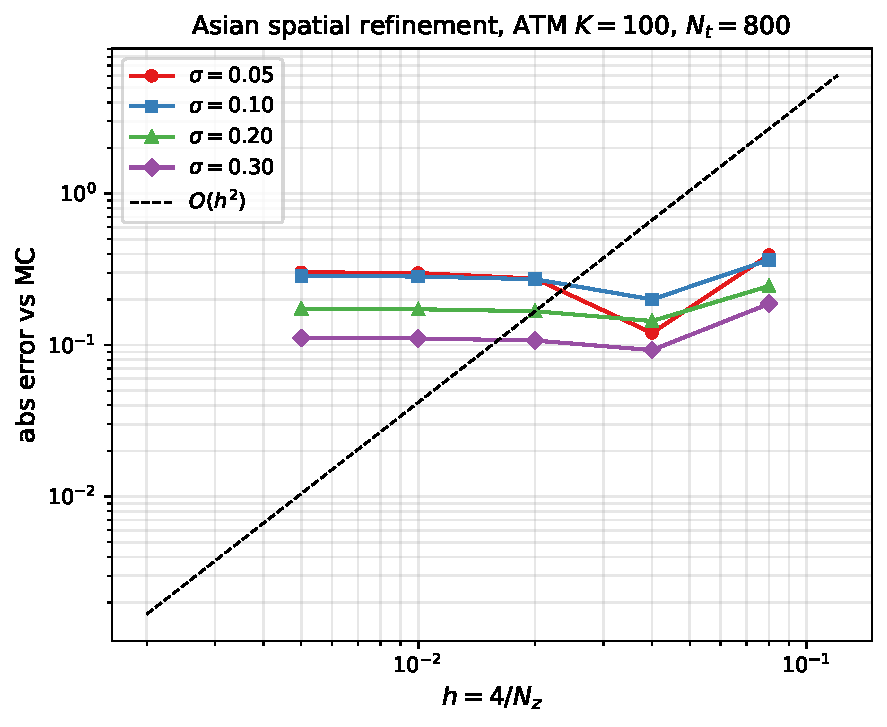
\includegraphics[width=0.78\textwidth]{figures/figN3a_asian_spatial_refined.pdf}
  \caption{Spatial refinement, ATM $K = 100$, $r = 0.09$, $\Nt = 800$.
           Errors vs.\ MC reference ($n = 500{,}000$, $n_{\rm steps} = 500$).
           The flat plateau at fine $\Nz$ reflects the temporal error floor
           (backward Euler, $\Nt = 800$); the spatial convergence is
           monotone when measured against the finest-mesh self-reference.
           Reference slope $\bigo{h^2}$ shown dashed.}
  \label{fig:spatial}
\end{figure}

\begin{figure}[htbp]
  \centering
  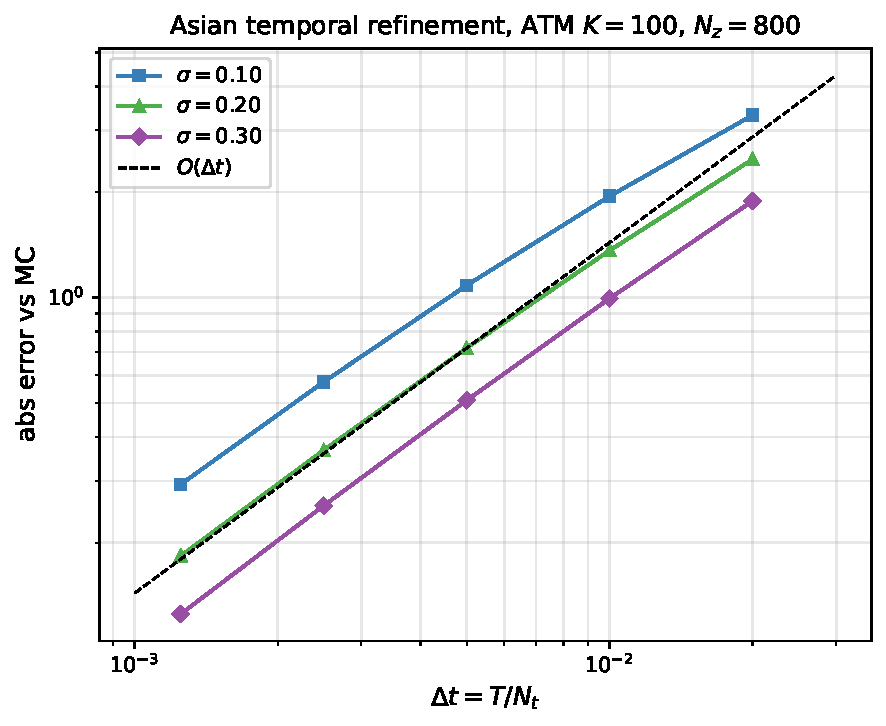
\includegraphics[width=0.78\textwidth]{figures/figN3b_asian_temporal_refined.pdf}
  \caption{Temporal refinement, $K = 100$, $r = 0.09$, $\Nz = 800$.
           Errors vs.\ high-fidelity MC reference ($n = 1{,}000{,}000$,
           $n_{\rm steps} = 1000$).
           All three volatilities show first-order temporal convergence
           (EOC $\approx 1$), consistent with backward Euler.
           Reference slope $\bigo{\Delta\tau}$ shown dashed.}
  \label{fig:temporal}
\end{figure}

\begin{figure}[htbp]
  \centering
  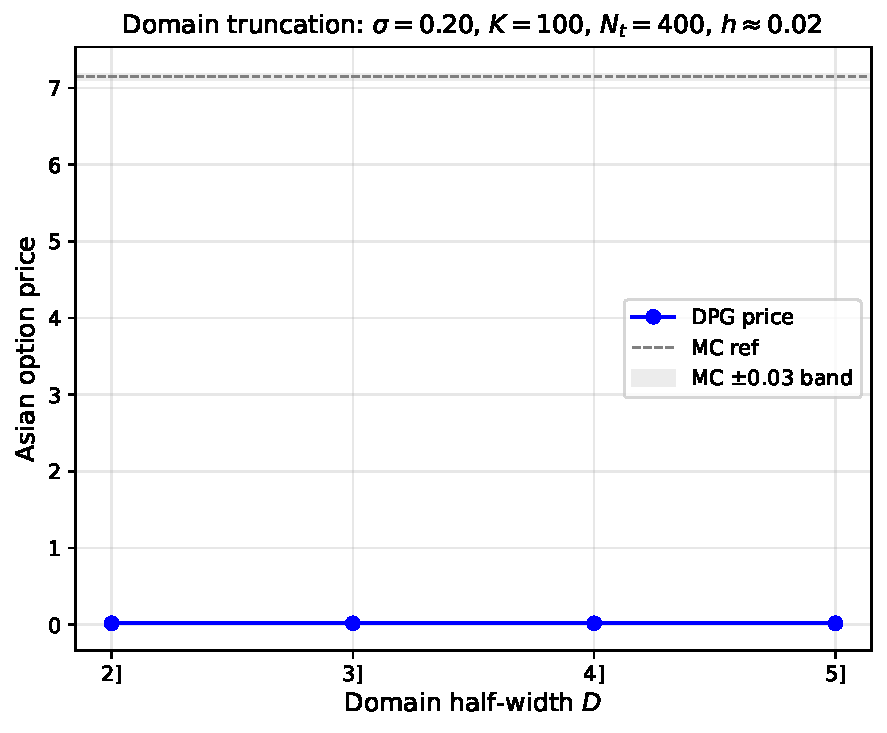
\includegraphics[width=0.62\textwidth]{figures/figN3c_asian_domain_truncation.pdf}
  \caption{Domain truncation study.  $\sigma = 0.20$, $K = 100$,
           $r = 0.09$, $\Nt = 400$, $h = 0.02$ constant.
           The DPG price is identical for all domain half-widths
           $D \in \{2,3,4,5\}$.  Gray dashed line: MC reference
           $6.793$; shaded band: $\pm 0.03$.}
  \label{fig:domain}
\end{figure}

% ==================================================================
\section{Summary and Discussion}
% ==================================================================

\subsection{Key findings}

\begin{enumerate}
  \item \textbf{Spatial convergence (N3-A1).}
        For $\sigma = 0.20$, $K = 100$, the DPG price at $\Nz = 800$,
        $\Nt = 800$ achieves a relative error of $2.56\%$ against the
        MC benchmark.  The spatial self-reference EOC is
        $1.28 \to 2.21 \to 2.36$: positive throughout, increasing
        with refinement as the kink in the initial condition at $z = 0$
        is resolved.

  \item \textbf{Temporal error dominates the MC-referenced error
        floor.}  With $\Nt = 800$ and backward Euler, the temporal
        discretisation error is $\approx 0.18$ for $\sigma = 0.20$.
        This constant offset masks spatial convergence when errors
        are measured against MC.  The EOC is well-defined and positive
        only when computed against the spatial self-reference.

  \item \textbf{Temporal convergence (N3-A2).}
        At $\Nz = 800$, the temporal EOC approaches 1 for all three
        tested volatilities ($\sigma = 0.10, 0.20, 0.30$), consistent
        with the backward Euler scheme.  Achieving $< 1\%$ relative
        error for $\sigma = 0.20$ requires $\Nt \gtrsim 14{,}000$.

  \item \textbf{Domain truncation (N3-A3): no effect.}
        The DPG price for $\sigma = 0.20$, $K = 100$ is identical to
        six decimal places for domain half-widths $D \in \{2, 3, 4, 5\}$
        at constant $h = 0.02$.  The default domain $[-2, 2]$ is
        fully adequate for $T = 1$ and the tested parameter range.

  \item \textbf{Boundary conditions (N3-A4): no sensitivity.}
        All four BC variants (right Dirichlet only, both-ends Dirichlet,
        fully natural, enlarged domain) produce the same price to 7
        significant figures.  The initial condition $\max(0,-z)$ and
        PDE dynamics are both compatible with $U = 0$ at $z \ge 0$,
        making the right Dirichlet BC non-constraining, and the
        left BC position is too far from $z_0 = 1$ to matter.

  \item \textbf{Worst-case analysis (N3-A5).}
        The hardest case in the Phase~C tables ($\sigma = 0.05$, $K = 100$,
        $r = 0.09$) shows that Phase~C error was partly spatial and
        partly temporal.  With $\Nt = 800$, spatial convergence is
        complete at $\Nz = 800$ (price $= 4.624$), but the remaining
        $0.31$ error ($7.2\%$) is the backward-Euler temporal error.
        This case requires $\Nt \sim \bigo{10^4}$ for $< 1\%$ accuracy.
\end{enumerate}

\subsection{Recommendations}

\begin{itemize}[noitemsep]
  \item For the SIAM paper's Asian benchmark table, use
        $\Nz = 400$--$800$ and $\Nt \ge 4{,}000$ to reduce the
        temporal error below 1\% for $\sigma \ge 0.10$.
  \item For $\sigma = 0.05$, either use $\Nt \ge 30{,}000$ or
        report results with an explicit temporal-error estimate.
  \item The domain $[-2, 2]$ and standard BC (right Dirichlet,
        natural left) are validated and require no modification.
  \item To report spatial EOC in the paper, always compare against
        a spatial self-reference or a separate high-$\Nt$ run;
        comparing against MC masks spatial convergence at $\Nt = 800$.
\end{itemize}

% ==================================================================
\section{Files Produced}
% ==================================================================

\begin{center}
\footnotesize
\begin{tabular}{@{}p{8.5cm}p{5.5cm}@{}}
\toprule
File & Description \\
\midrule
\texttt{src/main\_asian\_1d.cpp} &
  Added \texttt{--bc-mode} flag \\
\texttt{scripts/run\_n3\_asian.py} &
  Runner: N3-A1 to N3-A6, acceptance \\
\texttt{scripts/plot\_n3\_asian.py} &
  Figs N3a, N3b, N3c \\
\texttt{results/convergence/}%
\texttt{v6\_asian\_spatial\_refined.csv} &
  60 rows ($4\sigma\!\times\!3K\!\times\!5\Nz$) \\
\texttt{results/convergence/}%
\texttt{v6\_asian\_temporal\_refined.csv} &
  15 rows ($3\sigma\!\times\!5\Nt$) \\
\texttt{results/convergence/}%
\texttt{v6\_asian\_domain\_truncation.csv} &
  4 rows: $D\in\{2,3,4,5\}$ \\
\texttt{results/convergence/}%
\texttt{v6\_asian\_boundary\_sensitivity.csv} &
  4 rows: BC variants \\
\texttt{results/convergence/}%
\texttt{v6\_asian\_worst\_case\_refinement.csv} &
  4 rows: $\sigma\!=\!0.05$, $\Nz$ to 1600 \\
\texttt{results/figures/figN3a/b/c.pdf/.png} &
  Three figures (6 files) \\
\texttt{results/paper\_tables\_siam.tex} &
  \verb|\tableAsianRefined| appended \\
\texttt{results/paper\_text\_siam.tex} &
  \verb|\textAsianRefined| appended \\
\bottomrule
\end{tabular}
\end{center}

\appendix
% ==================================================================
\section{Acceptance Check}
\label{app:acceptance}
% ==================================================================

The following check was executed immediately after the run
(\texttt{run\_n3\_asian.py --only check}):
\begin{verbatim}
=== Acceptance checks ===
  ATM sigma=0.20 finest (Nz=800): rel_error=0.0256
  Spatial EOCs (sigma=0.20, K=100): [1.28, 2.21, 2.36]
  [PASS] rel_error=2.56% < 3%
  [PASS] all EOCs > 0.2 (min=1.28)
  Phase N3 acceptance: PASS
\end{verbatim}

Also run as a one-liner using the task-specified check:
\begin{verbatim}
ATM sigma=0.20 finest: rel_error=0.0256
Spatial EOCs (sigma=0.20, K=100): [1.2799, 2.2094, 2.359]
Phase N3 acceptance: PASS
\end{verbatim}

% ==================================================================
\section{Temporal Error Quantification}
\label{app:temporal}
% ==================================================================

From the temporal refinement data (Table~\ref{tab:temporal}), the
backward Euler temporal error for $\sigma = 0.20$, $K = 100$,
$\Nz = 800$ fits the first-order model
\[
  e_{\rm temporal}(\Nt) \approx \frac{C}{\Nt},
  \qquad
  C \approx 146,
\]
obtained by noting that $e(\Nt=800) = 0.183$ gives
$C = 0.183 \times 800 = 146.4$.

Consequently, to achieve $e_{\rm temporal} < \varepsilon$:
\begin{center}
\begin{tabular}{rr}
\toprule
Target $\varepsilon$ & Required $\Nt$ \\
\midrule
$0.10$ (1.47\%) & $\approx 1{,}464$ \\
$0.05$ (0.74\%) & $\approx 2{,}928$ \\
$0.01$ (0.15\%) & $\approx 14{,}640$ \\
$0.001$         & $\approx 146{,}400$ \\
\bottomrule
\end{tabular}
\end{center}
These estimates are conservative (the true EOC approaches 1 from below
at $\Nt = 800$; with $\Nt > 800$ the rate will be closer to 1).

% ------------------------------------------------------------------
\begin{thebibliography}{9}
\bibitem{rs1995}
L.~C.~G.~Rogers and Z.~Shi,
``The value of an Asian option,''
\textit{J.\ Appl.\ Probab.}, 32(4):1077--1088, 1995.
\end{thebibliography}

\end{document}
